\chapter{Conceptualisation and Modelling}
\label{chp2:concept_model}


\section{System Concepts}
%WHAT you are going to present in this chapter/section
%WHY you are presenting it, and
%HOW you are going to present it
The report contains many variable names and use of terminology for concepts that is used throughout the report. These variables and terminologies are defined here.\\

The double pendulum is a under-actuated system which is defined as a system where the input to the system cannot command any of the state variables an instantaneous acceleration. This is due to the torque input only actuating the lower pendulum and the energy in the lower pendulum must be transferred to the upper pendulum to initiate an acceleration. \\

The robotic gymnast is describe as a double pendulum consisting out of an actuated- and non-actuated pendulum as seen in Figure \ref{fig:doublePen}. The position of the non-actuated pendulum is described by the angle $\theta$ whereas the actuated pendulum is described by $\phi$ relative to $\theta$. The angle's $\theta$ and $\phi$ are the independent parameters that describe the entire system.\\

There are 2 position of interest where the system contain special characteristics. These 2 positions are the stable- and unstable equilibrium position. In the stable position the system is at rest hanging downward when $\theta = \SI{0}{\radian}$ and $\phi = \SI{0}{\radian}$. It is stable due to the having negative real poles resulting in the system returning to this position when disturbed. The unstable equilibrium position is where $\theta=\SI{2\pi}{\radian}$ and $\phi = \SI{0}{rad}$ resulting in the robotic gymnast balancing upside down. In this position the system contain positive real poles and any disturbance will cause the system to exponentially grow away from this position.\\

region of controllability:he null controllability region is the set of states that can be steered to inverted unstable equilibrium position in a fixed time with a constrained control input \cite{null_controllability}.

LTI system


\section{Mathematical Model}
\label{sec:math_model}
%WHAT you are going to present in this chapter/section
%WHY you are presenting it, and
%HOW you are going to present it
\begin{figure}[h]
	\centering
	\input{"./figs/freebodydiagram/doublePendulumImage.tikz"}
	\caption{Free Body Diagram of the Double Pendulum}
	\label{fig:doublePen}
\end{figure}

The approach taken to derive the mathematical model of the robotic gymnast will be discussed in this section. It is presented to allow the reader to understand parameters mentioned in the report. The swing-up of the robotic gymnast consist of non-linear behaviour and is require to fully derive the dynamics of the system. The strenuous mathematical steps are removed from the reader, which is provided in Appendix \ref{sec:math_model}, and a summary of the motivation and paradigm approach to the derivation is provided here.\\

The robotic gymnast is modelled as two pendulums connected together with a hinge, where each pendulum is modeled as having their mass distributed arbitrary along their axis. There is a torque actuating the lower pendulum seen in Figure \ref{fig:doublePen} and friction is modelled as proportional to the angular velocity of the pendulums. The friction that develops at the hinge is proportional to the relative motion of the actuated pendulum and non-actuated pendulum. The angle, $\phi$ was purposefully chosen relative to $\theta$ to ease the identification of this friction. Figure \ref{fig:doublePen} displays the free body diagram of the robotic gymnast.\\

Deriving the equation of motion of the robotic gymnast can be approached using different methods. The method chosen in the report is by using the Euler-Lagrange equation. The Euler-Lagrange equation shown in (\ref{eq:euler_lagrange_expanded}) derives the dynamics of the system by analysing the energy of the system.  This approach was chosen due to the energy of the system being easily defined as the potential energy $T$ of the 2 pendulums, and the kinetic energy $V$ of the pendulums.
 
\begin{equation} \label{eq:euler_lagrange_expanded}
\frac{d}{dt}\frac{\partial\mathcal{L}}{\partial\vec{\dot{q}}}-\frac{\partial\mathcal{L}}{ \vec{\partial q}} = 0
\end{equation}

\begin{equation} \label{eq:euler_lagrane}
\mathcal{L}=T-V
\end{equation}

Using the Euler-Lagrange equation leads to the condense equations shown in (\ref{eq:condense1}) and (\ref{eq:condense2}),
\begin{equation} \label{eq:condense1}
d_{11}\ddot{\theta}+d_{12}\ddot{\phi} + h_{1} + \psi_{1} = 0
\end{equation}
\begin{equation} \label{eq:condense2}
d_{21}\ddot{\theta} + d_{22}\ddot{\phi} + h_{2} + \psi_{2} = \tau
\end{equation}
where the coefficients are defined as
\begin{equation} \label{eq:d11}
d_{11} = I_{a} + I_{b} + m_{2}(L_{1}^2 + l_{2}^2+2L_{1}l_{2}\cos(\phi))
\end{equation}
\begin{equation} \label{eq:d12}
d_{12} = I_{b} +m_{2}(l_{2}^2 L_{1}l_{2}\cos(\phi))
\end{equation}
\begin{equation} \label{eq:h1}
h_{1} = -m_{2}L_{1}l_{2}\sin(\phi)\dot{\phi^2}-2m_{2}L_{1}l_{2}\sin(\phi)\dot{\phi}\dot{\theta}
\end{equation}
\begin{equation} \label{eq:psi1}
\psi_{1} = (m_{2}l_{1}+m_{2}L_{1})g\cos(\theta) + m_{2}l_{2}g\cos(\theta+\phi) + f_{c_{1}}
\end{equation}
\begin{equation} \label{eq:d21}
d_{21}= I_{b}+m_{2}(l_{2}^2+L_{1}l_{2}\cos(\phi))
\end{equation}
\begin{equation} \label{eq:d22}
d_{22}= I_{b}+ m_{2}l_{2}^2
\end{equation}
\begin{equation} \label{eq:h2}
h_{2}= m_{2}L_{1}l_{2}\sin(\phi)\dot{\theta^2}
\end{equation}
\begin{equation} \label{eq:psi2}
\psi_{2}= m_{2}l_{2}g\cos(\theta+\phi) + f_{c_{2}}
\end{equation}

\section{Simulation Model}
	%WHAT you are going to present in this chapter/section
%WHY you are presenting it, and
%HOW you are going to present it
The mathematical model derived in the previous section is required to be implemented on a simulation program. Simulating the model allows the designer to understand how system parameters influence the dynamics of the system and the verification of controllers implemented. It will be presented by discussing how the simulation is a true representation of the system, how design specifications were determined and the influence of these parameters.\\

Simulation of the robotic gymnast was done using MATLAB Simulink. The differential equations shown in equation (\ref{eq:condense1}) and (\ref{eq:condense2}) were implemented using the MATLAB function box. It was required to write $\ddot{\phi}$ and $\ddot{\theta}$ as the subject in each of the \textit{MATLAB Function} box to allow MATLAB to simulate the model.\\

Other non-linearities introduced by sensors and components were added such as saturation of the motor, gearbox backlash and quantisation of sensory data. These non-linearities were implemented to allow the simulation to be an acceptable representation of the physical system. The Simulink Model is shown in Figure \ref{fig:sim_nonlinearfeedback}.

\begin{figure}[h]
	\centering
	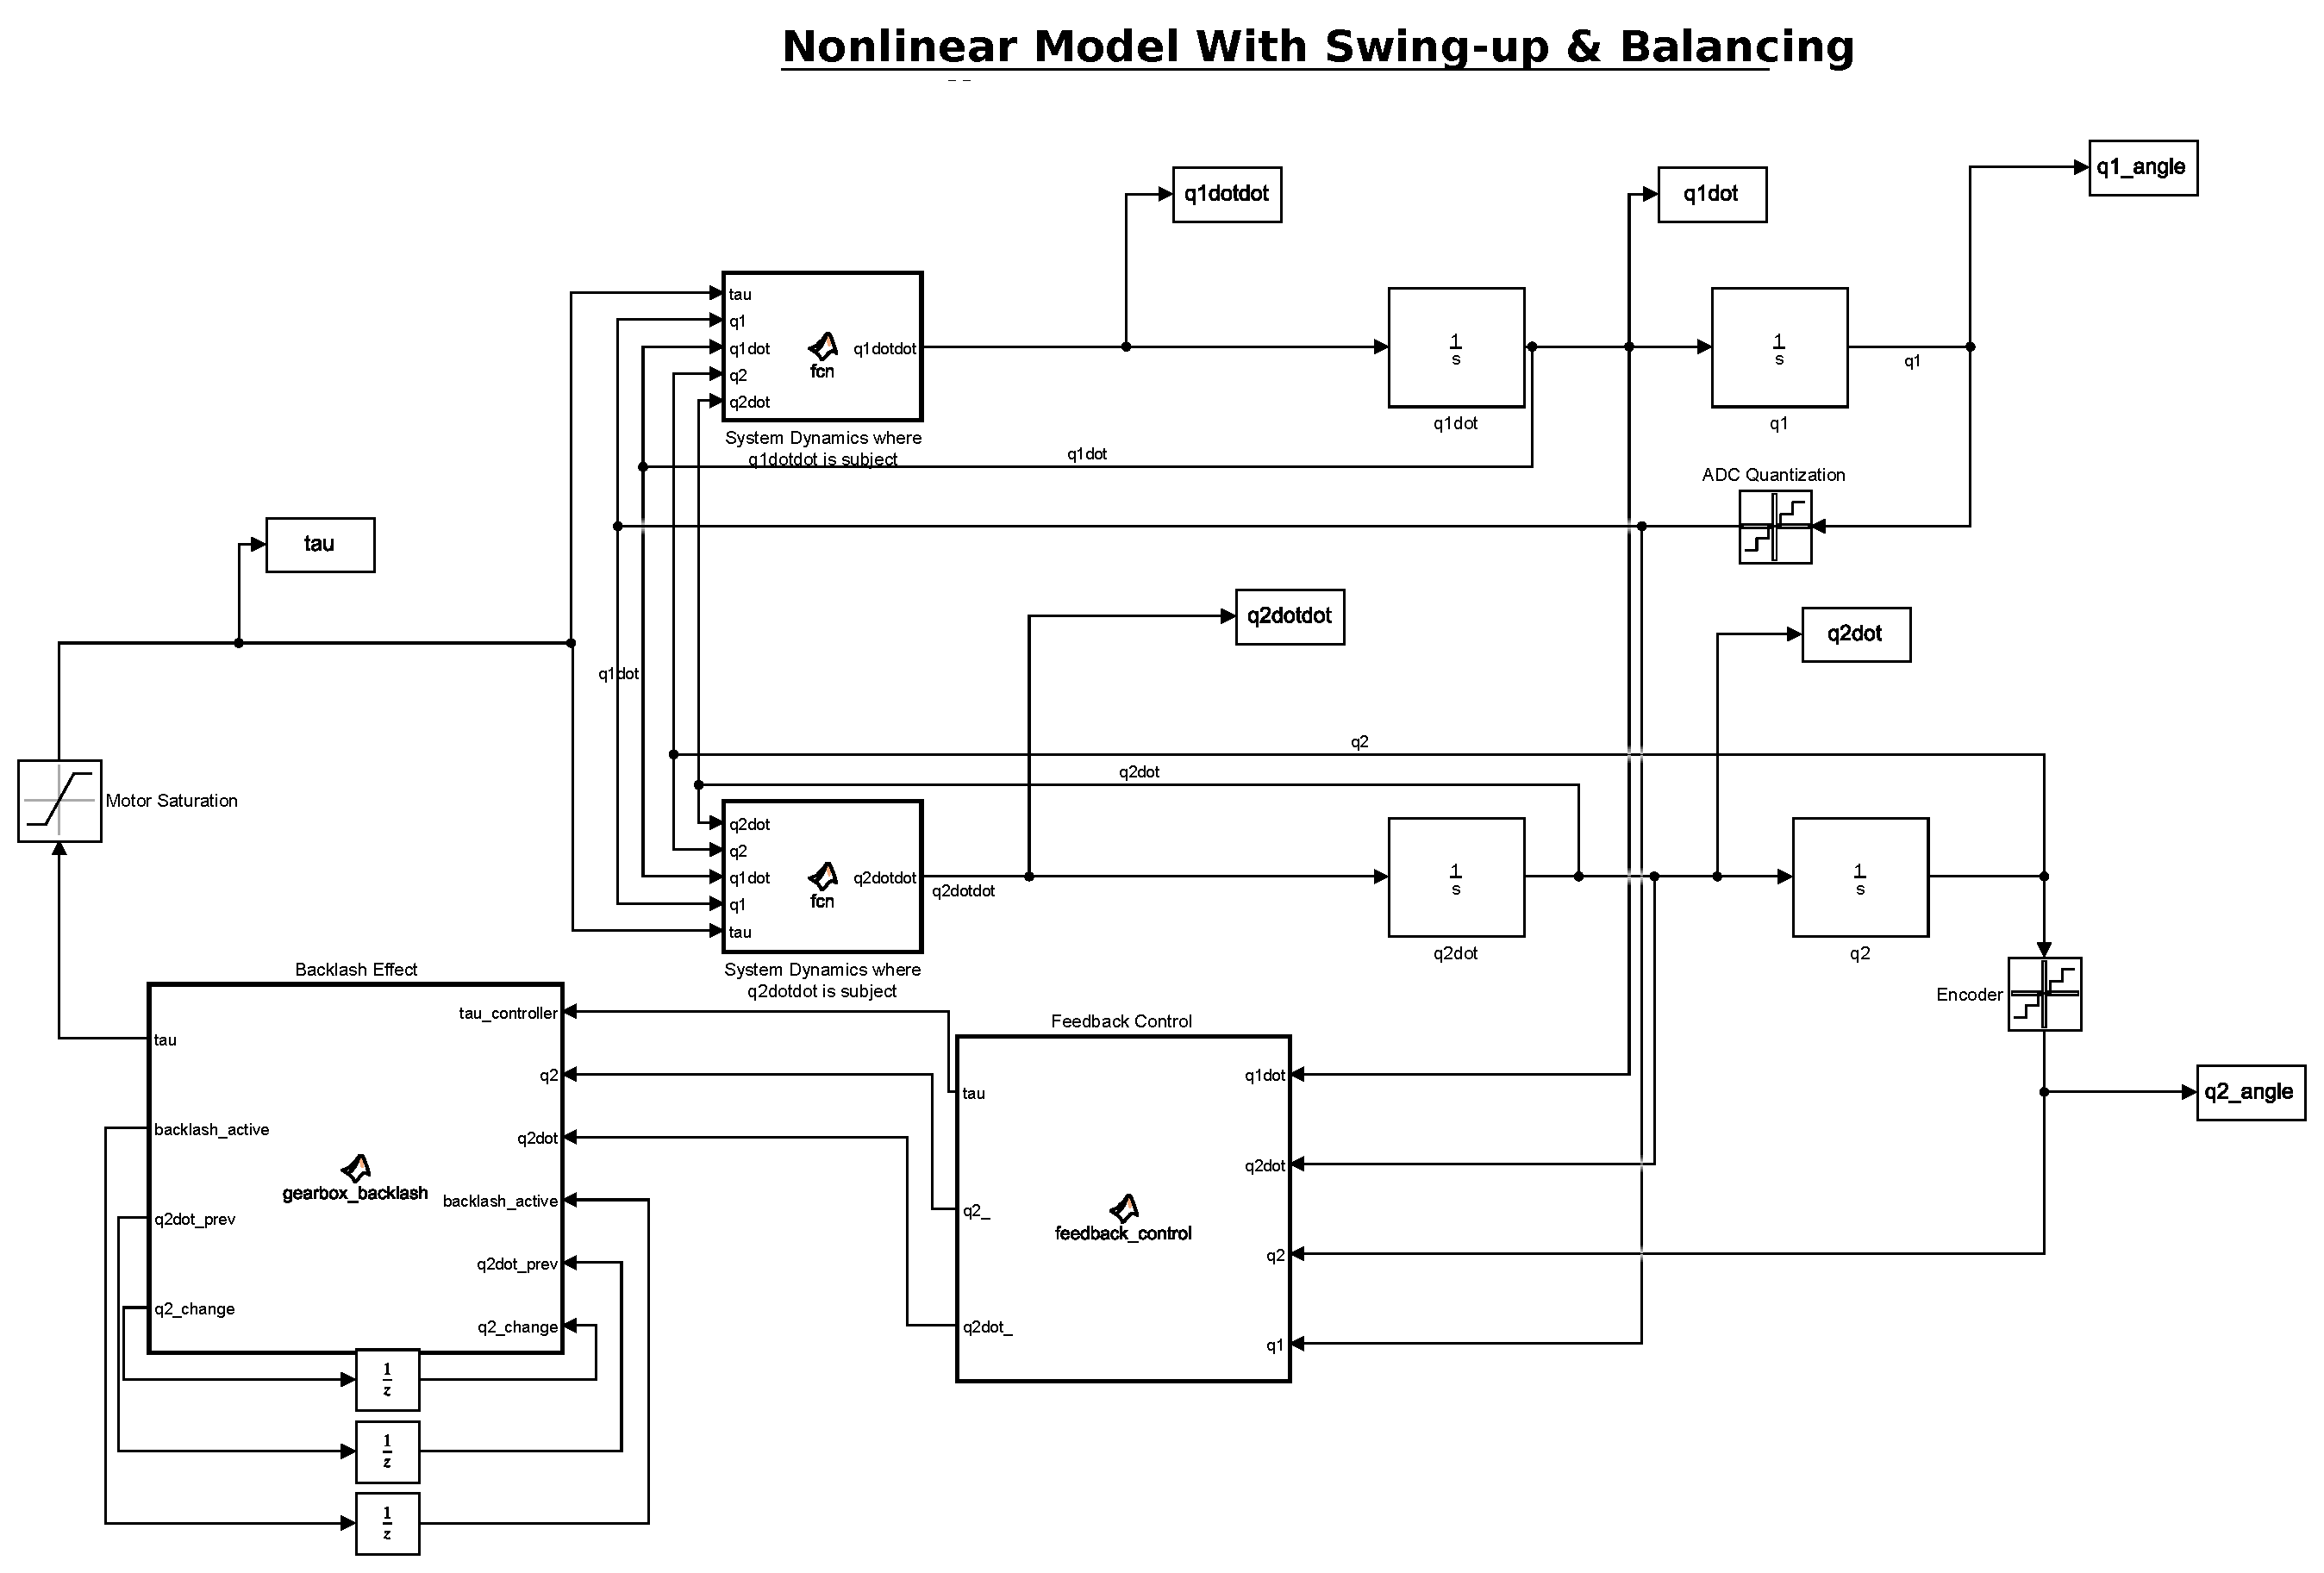
\includegraphics[scale=0.3]{./figs/simulink/simulink_model.eps}
	\caption{MATLAB Simulink Model}
	\label{fig:sim_nonlinearfeedback}
\end{figure}

\section{System Identification}
%WHAT you are going to present in this chapter/section
%WHY you are presenting it, and
%HOW you are going to present it?

The system identification tests are done to determine the characteristics that describe the behavior of the system. These characteristics include the damping ratio's and natural frequencies of the system. These characteristics will be presented by showing measured responses and how these responses can be modelled. \\

The project started off with a previous physical model which provided realistic system parameters to allow the simulation to be an acceptable representation of a physical model. From using these previous system parameters the simulation provided a set of specification for the new mechanical design. All responses shown and values calculated are based of the new mechanical design parameters shown in Table \ref{table:system_param} throughout the report.\\


		\begin{table}[]
	\centering
	\begin{tabular}{|c|c|}
		\hline
		System Parameter & Value \\
		\hline
		\hline
		$L_{1}$ & \SI{0.235}{m} \\
		\hline
		$L_{2}$ & \SI{0.314}{m} \\ 
		\hline
		$I_{A}$ & \SI{ 0.0022}{kg\cdot m^2}\\
		\hline
		$I_{B}$ & \SI{0.0054}{kg\cdot m^2}\\
		\hline
		$m_{1}$ & \SI{0.576}{kg}\\
		\hline
		$m_{2}$ & \SI{0.492}{kg} \\
		\hline
		$l_{1}$ & \SI{0.205}{m}\\
		\hline
		$l_{2}$ & \SI{0.238}{m}\\
		\hline
	\end{tabular}
	\caption{System Parameters}
	\label{table:system_param}
\end{table}


Since the system is described by 2 independent parameters the system is thus a 2 degree of freedom (2DOF) system and is expected to contain 2 natural frequencies each accompanied by a damping coefficient. The first natural frequency of the system was determine by inspecting the response of the system when starting at a initial condition and keeping $\phi = \SI{0}{\radian}$ constant throughout the response. This was done by using a lightweight PVC pipe that has negligible effect on the weight of the system. The actuated pendulum and non-actuated pendulum are constrained to this pipe to ensure the 2 pendulums stay in-line with each other and thus ensuring $\phi = \SI{0}{\radian}$. The response of the system is shown in Figure \ref{fig:q1_response} starting at a initial condition of roughly $\theta = \frac{\pi}{6}$. The accuracy of the initial conditions is of little importance, but the initial condition must allow the response to contain a few oscillation to accurately determine the parameter of interest.\\

\begin{figure}[h]
	\centering
	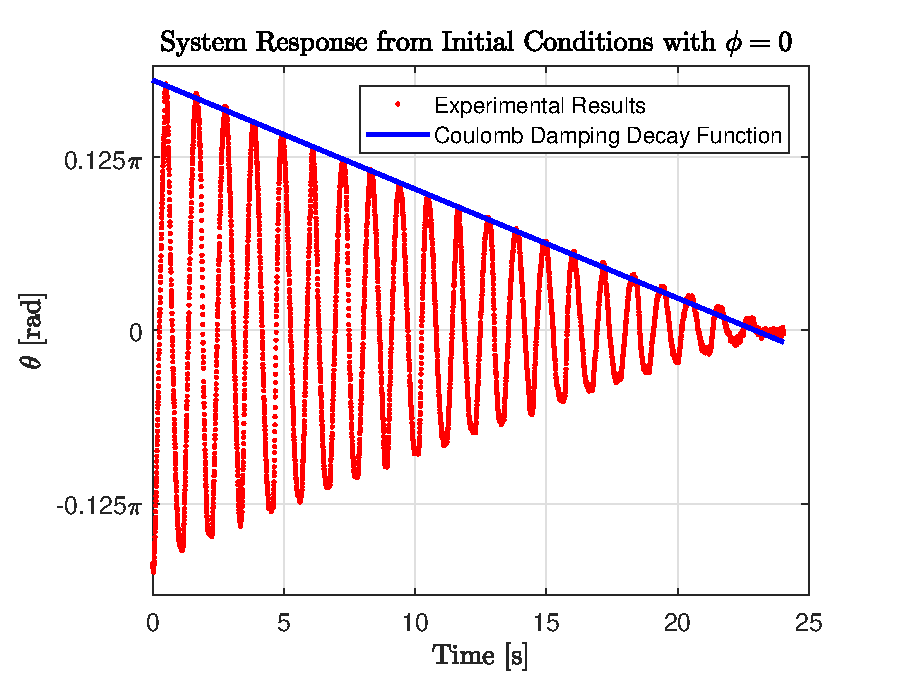
\includegraphics[scale=1]{./figs/q1_initial_response.eps}
	\caption{Initial Condition System Response while $ \phi = \SI{0}{rad} $ }
	\label{fig:q1_response}
\end{figure}


The second natural frequency is determined by analysing the response of the system when $\phi$ starts at a initial condition and keeping $\theta = \SI{0}{\radian}$ throughout the response. This was accomplished by constraining the non-actuated pendulum using hard stops. Figure \ref{fig:q2_response} shows the measured response of the system when $\phi$ starts at a initial condition and keeping $\theta = \SI{0}{\radian} $.\\

\begin{figure}[h]
	\centering
	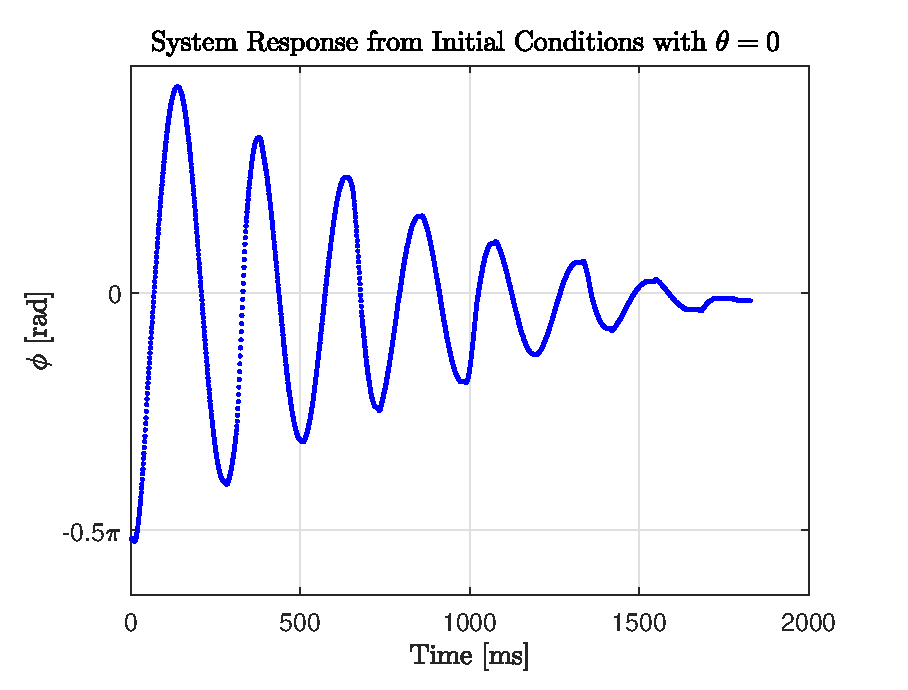
\includegraphics[scale=1]{./figs/q2_initial_response.eps}
	\caption{Initial Condition System Response while $ \theta = \SI{0}{rad} $ }
	\label{fig:q2_response}
\end{figure}

The damped natural frequencies of the system was identified by inspecting the frequency content of the time-domain responses. The frequency content of the initial condition responses of both experiments are shown in Figure \ref{fig:fft_system_response}, by applying the Fast Fourier Transform (FFT) algorithm to the time-domain signals. The FFT indicates the damped natural frequencies by the predominant peaks across the frequency spectrum which are tabulated in Table \ref{table:system_characteristic}.\\

\begin{figure}[h]
	\centering
	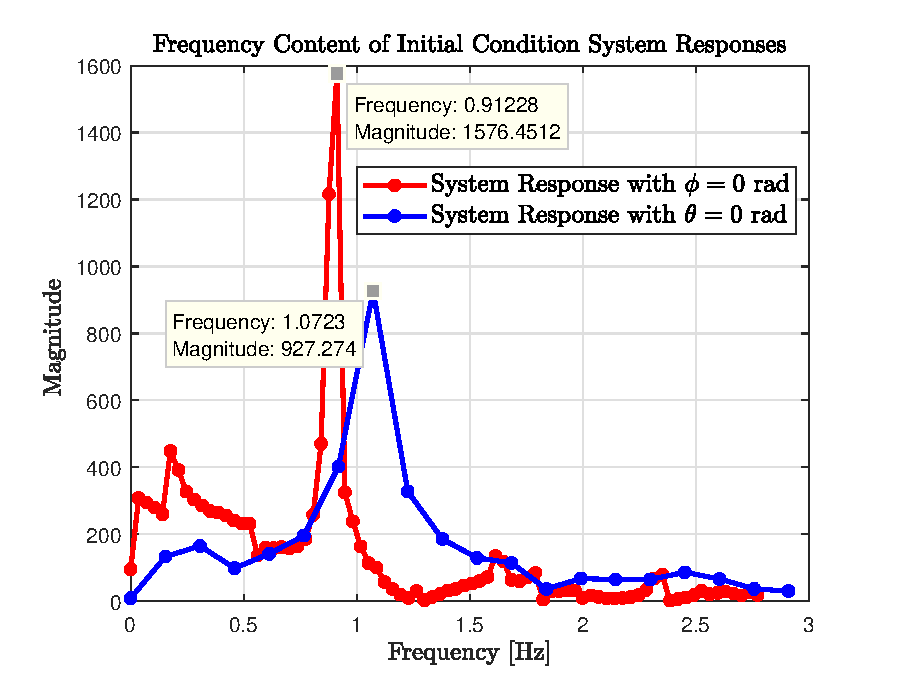
\includegraphics[scale=1]{./figs/FFT_system.eps}
	\caption{Frequency Content of Time-Domain Initial Condition Responses}
	\label{fig:fft_system_response}
\end{figure}

The response shown in Figure \ref{fig:q1_response} is under the influence of coulomb damping due to the response being characterised by the amplitude decaying linearly with a constant slope. Coulomb damping is caused by sliding friction and it's force is opposite to the direction of velocity \citep{coulomb_friction}. It is thus characterised as  $$ f_{c_{1}} = 
\left \{
\begin{tabular}{cc}
$ -\mu N $ & $ \dot{\theta}> 0 $\\
$ 0 $ & $ \dot{\theta} = 0$\\
$\mu N &   $ \dot{\theta} < 0$ \\
\end{tabular}
\right \}
$$

It is shown in \citet{coulomb_friction} that the slope is defined as 
\begin{equation} \label{eq:coulomb_slope}
-\frac{2\mu N \omega_{n}}{\pi mg}
\end{equation}
where $N$  is the normal force. The slope seen in the decay function in Figure \ref{fig:q1_response} was calculated using linear regression and by knowing the terms in equation \ref{eq:coulomb_slope} the combined $\mu N$ term can be calculated and is shown in Table \ref{table:system_characteristic}.\\

The responses shown in Figure \ref{fig:q2_response} is decaying exponentially with time and this decaying behaviour can be modelled by the following equation: $$\tau(t) = -\zeta \omega_{n} t$$ Where $\omega_{n}$ is the natural frequency and $\zeta$ the damping ratio of the system. The damped natural frequencies of the system has already been determined and thus linear regression can be used to determine the best $\zeta$ that will fit the measured data. The decaying function is shown in Figure \ref{fig:q2_response} with the $\zeta$ value shown in Table \ref{table:system_characteristic}. It is visible from the response that the damping ratio fits the data well and only starts to deviate near steady state. The damping force, $f_{c_{2}}$ can be characterised as $2\zeta\omega_{n}$ due to response shown in Figure \ref{fig:q2_response} being describe as second order differential equation. 

\begin{table}[]
	\centering
	\begin{tabular}{|c|c|c|c|}
		\hline
		System Characteristic & Mean & Standard Deviation\\
		\hline
		\hline
		$f_{1}$ & \SI{0.906}{Hz} & 0.014 \\
		\hline
		$f_{2}$ & \SI{1.081}{Hz} & 0.044 \\ 
		\hline
		$\mu N$ & $ $ & $ $
		\\
		\hline
		$\zeta_{2}$ &  & \\
		\hline
	\end{tabular}
	\caption{System Characteristic \& their Statistical Properties from 5 Experiments}
	\label{table:system_characteristic}
\end{table}

\section{Model Validation}
%WHAT you are going to present in this chapter/section
%WHY you are presenting it, and
%HOW you are going to present it?
The model implemented in simulation must be able describe the physical model to an acceptable degree to allow any further development on the simulated model. The simulated model will be validated by comparing the experimental system characteristic values to those attained in simulation and proof that the simulated model is an accurate representation of the physical model.\\

Table \ref{table:experiment_vs_simulation} shows the experimental values determined in the previous section against the simulation characteristic and indicates the simulation model represents the physical model well. Figure \ref{fig:sim_vs_measured_q1} and \ref{fig:sim_vs_measured_q2} provides an visually verification that the damping effects are modelled to an acceptable degree.\\

The proof indicates the physical model is well represented and further developments on the simulated model may occur.\\



 
\begin{table}[]
	\centering
	\begin{tabular}{|c|c|c|c|c|}
		\hline
		System & $\omega_{n_{1}}$  & $\omega_{n_{2}}$  & $\zeta_{1}$ & $\zeta_{2}$ \\
		\hline
		\hline
		Experimental  & 5.692 &  6.793 & & \\
		\hline
		Simulation & 5.654 & 6.704 & & \\ 
		\hline
	\end{tabular}
	\caption{Experimental Characteristics vs Simulation Model Characteristic}
	\label{table:experiment_vs_simulation}
\end{table}

\begin{figure}[h]
	\centering
	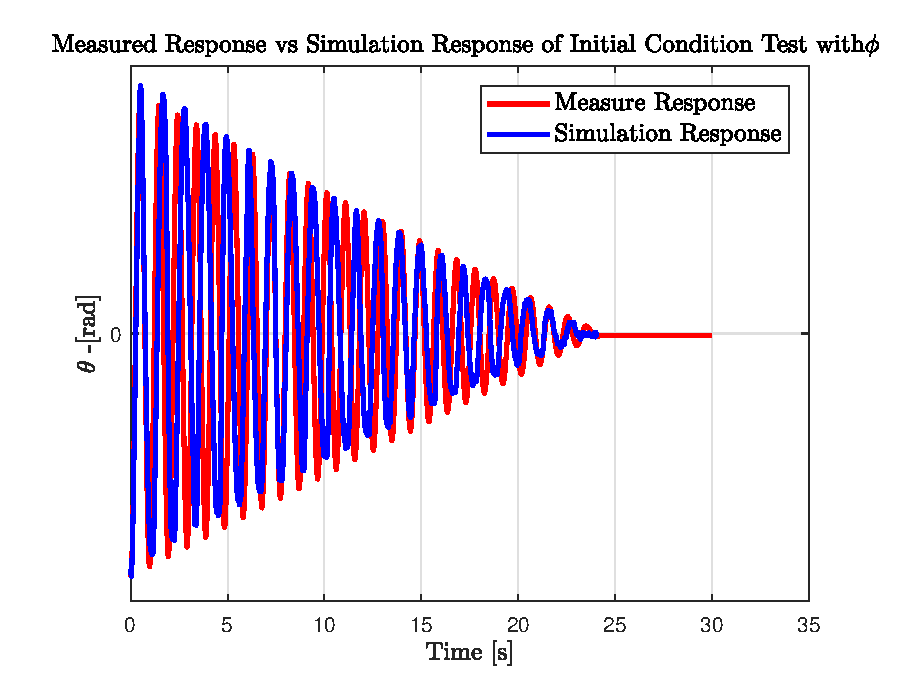
\includegraphics[scale=1]{./figs/sim_vs_measured_q1.eps}
	\caption{Comparison between Simulated and Measured Response}
	\label{fig:sim_vs_measured_q1}
\end{figure}


